\documentclass[11pt]{article}

\usepackage{amsmath,amsthm,amsfonts,amssymb,amsxtra}
\usepackage{pgf,tikz}
\usepackage{mathrsfs}
\renewcommand{\theenumi}{(\alph{enumi})} 
\renewcommand{\labelenumi}{\theenumi}

\pagestyle{empty}
\setlength{\textwidth}{7in}
\setlength{\oddsidemargin}{-0.5in}
\setlength{\topmargin}{-1.0in}
\setlength{\textheight}{9.5in}

\theoremstyle{definition}
\newtheorem{problem}{Problem}
\theoremstyle{theorem} 
\newtheorem*{theorem}{Theorem}
\newtheorem{proposition}{Proposition}


\begin{document}

\noindent{\large\bf MATH 300}\hfill{\large\bf Final Exam}\hfill{\large\bf Fall 2018}\hfill{\large\bf Page 1/6}\hrule

\bigskip
\begin{center}
  \begin{tabular}{|ll|}
    \hline & \cr
    {\bf Name: } & \makebox[12cm]{\hrulefill}\cr & \cr
    {\bf VIP ID:} & \makebox[12cm]{\hrulefill}\cr & \cr
    \hline
  \end{tabular}
\end{center}
\begin{itemize}
\item Write your name and VIP ID in the space provided above.
\item The test has six (6) pages, including this one.
\item Credit for each problem is given at the right of each problem number.
\item Show sufficient work to justify all answers unless otherwise stated in the problem.  Correct answers with
  inconsistent work may not be given credit.
\item No notes are allowed.  You may use your book and a graphing calculator (without Computer Algebra System) if
  needed.
\end{itemize}
\hrule

\begin{center}
  \begin{tabular}{|c|c|c|}
    \hline
    &&\cr
       {\large\bf Page} & {\large\bf Max}  & {\large\bf Points} \cr
    &&\cr
       \hline
    &&\cr
       {\Large 2} & \Large 20 &  \cr
    &&\cr
       \hline
    &&\cr
       {\Large 3} & \Large 25 & \cr
    &&\cr
       \hline
    &&\cr
       {\Large 4} & \Large 15 & \cr
    &&\cr
       \hline
    &&\cr
       {\Large 5} & \Large 20 & \cr
    &&\cr
       \hline
    &&\cr
       {\Large 6} & \Large 20 & \cr
    &&\cr
       \hline\hline
    &&\cr
       {\large\bf Total} & \Large 100 & \cr
    &&\cr
       \hline
  \end{tabular}
\end{center}
\newpage

%%%%%%%%%%%%%%%%%%%%%%%%%%%%%%%%%%%%%%%%%%%%%%%%%%%%%%%%%%%%%%%%%%%%% Page 2
\noindent{\large\bf MATH 300}\hfill{\large\bf Final Exam}\hfill{\large\bf Fall 2018}\hfill{\large\bf Page 2/6}\hrule

\bigskip
\begin{problem}[5 pts]
  Sketch the following set of points in the plane:
  \begin{equation*}
    \big\{ (x,y) \in \mathbb{R}^2 : (y-x^2)(y^2-x)(3-x) = 0 \big\}.
  \end{equation*}

  \vspace{4.5cm}
\end{problem}
\hrule

\begin{problem}[5 pts]\label{venn}
  Write the expression involving sets $A$, $B$ and $C$ given by the following Venn diagram:
  Write the expression involving sets $A$, $B$ and $C$ given by the following Venn diagram:
  \begin{center}
    \begin{tikzpicture}
      \draw[fill=gray] (330:1) circle (1.5);
      \draw[fill=white] (210:1) circle (1.5);
      % \draw[fill=white] (210:1) circle (1.5);
      \draw[fill=gray] ([shift=(185:1.5)]90:1) arc (185:295:1.5) -- ([shift=(5.264:1.5)]210:1) arc (5.264:114.73:1.5);      
      \draw (330:1) circle (1.5);
      \draw (90:1) circle (1.5);
      \draw (90:2.75) node{$B$};
      \draw (210:2.75) node{$A$};
      \draw (330:2.75) node{$C$};
    \end{tikzpicture}
  \end{center}

  \vspace{1cm}
\end{problem}
\hrule

\begin{problem}[10 pts--5 pts each part]
  Write the following sets either in set-builder notation, or by listing its elements.  Draw both sets on the plane.
  \begin{enumerate}
  \item $\displaystyle{\bigcup_{\alpha \in [0,2]}[\alpha,2] \times [0,5\alpha^2]=}$
  \item $\displaystyle{\bigcap_{\alpha \in [0,2]}[\alpha,2] \times [0,5\alpha^2]=}$
  \end{enumerate}
\end{problem}

\newpage

%%%%%%%%%%%%%%%%%%%%%%%%%%%%%%%%%%%%%%%%%%%%%%%%%%%%%%%%%%%%%%%%%%%%% Page 3
\noindent{\large\bf MATH 300}\hfill{\large\bf Final Exam}\hfill{\large\bf Fall 2018}\hfill{\large\bf Page 3/6}\hrule

\bigskip

\begin{problem}[5 pts]
  Decide whether or not the following two statements are logically equivalent:
  \begin{equation*}
    (\lnot P) \land (P \implies Q) \text{ and } \lnot ( Q \implies P)
  \end{equation*}

  \vspace{2cm}
\end{problem}
\hrule

\begin{problem}[5 pts]
  Give a statement that is logically equivalent to $\lnot (P \implies Q)$ that does not use the symbol $\lnot$.

  \vspace{3cm}
\end{problem}
\hrule

\begin{problem}[5 pts]
  Suppose that $P$, $Q$ and $R$ are statements and $(P \lor Q) \land (Q \implies R)$ is true.  If $R$ is false, give all
  possible combination of truth values of $P$ and $Q$ that work, or state that these cannot be determined.

  \vspace{4cm}
\end{problem}
\hrule

\begin{problem}[10 pts--5 pts each part]
  Consider the following statement $S$:
  \begin{quote}
    Given a real number $\varepsilon > 0$, there is a real number $\delta>0$ so that for all $x \in \mathbb{R}$, if $ 0
    < \lvert x-a \rvert < \delta$, then $\lvert f(x) - L \rvert < \varepsilon$.
  \end{quote}
  \begin{enumerate}
  \item Express $S$ in symbolic form.
    \vspace{3cm}
  \item Express $\lnot S$ in symbolic form without using the symbol $\lnot$.
  \end{enumerate}
\end{problem}
\newpage

%%%%%%%%%%%%%%%%%%%%%%%%%%%%%%%%%%%%%%%%%%%%%%%%%%%%%%%%%%%%%%%%%%%%% Page 4
\noindent{\large\bf MATH 300}\hfill{\large\bf Final Exam}\hfill{\large\bf Fall 2018}\hfill{\large\bf Page 4/6}\hrule

\bigskip
\begin{problem}[5 pts]
  Prove the following result:
  \vspace{-0.75cm}
  \begin{quotation}
    \begin{theorem}
      If $x \in \mathbb{R}$ and $0 < x < 3/2$, then $8x(3-2x) \leq 9$.
    \end{theorem}
  \end{quotation}

  \vspace{9cm}
\end{problem}
\hrule

\begin{problem}[10 pts--5 pts each part]
  Prove the following result:
  \vspace{-0.75cm}
  \begin{quotation}
    \begin{theorem}
      If the equation $ax^2+bx+c=0$ has two different real-valued solutions, and $b\neq 0$, then
      \begin{enumerate}
      \item The reciprocal of the sum of the two solutions is equal to $-a/b$.
      \item The product of the two solutions is equal to $c/a$.
      \end{enumerate}
    \end{theorem}
  \end{quotation}
\end{problem}
\newpage

%%%%%%%%%%%%%%%%%%%%%%%%%%%%%%%%%%%%%%%%%%%%%%%%%%%%%%%%%%%%%%%%%%%%% Page 5
\noindent{\large\bf MATH 300}\hfill{\large\bf Final Exam}\hfill{\large\bf Fall 2018}\hfill{\large\bf Page 5/6}\hrule

\bigskip
\begin{problem}[20 pts--10 pts each part]
  Prove the following propositions
  \vspace{-1cm}
  \begin{quotation}
    \begin{proposition}
      For every $n \in \mathbb{N},$ it follows that 
      \begin{equation*}
        \frac{1}{n} + \frac{1}{n+1} + \dotsb + \frac{1}{2n} \geq \frac{1}{2}. 
      \end{equation*}
    \end{proposition}
  \end{quotation}
  \vspace{9.5cm}
  \hrule
  \begin{quotation}
    \begin{proposition}
      Suppose $x,y \in \mathbb{R}.$  Then $x^3+x^2y=y^2+xy$ if and only if $y=x^2$ or $y+x=0$.
    \end{proposition}
  \end{quotation}
\end{problem}
\newpage

%%%%%%%%%%%%%%%%%%%%%%%%%%%%%%%%%%%%%%%%%%%%%%%%%%%%%%%%%%%%%%%%%%%%% Page 6
\noindent{\large\bf MATH 300}\hfill{\large\bf Final Exam}\hfill{\large\bf Fall 2018}\hfill{\large\bf Page 6/6}\hrule

\bigskip
\begin{problem}[10 pts--5 pts each part]
  Consider the function $f: \mathbb{Z} \times \mathbb{Z} \to \mathbb{Z}$ given by $f(m,n) = 7m + 2n$. Prove or disprove
  the following statements:
  \begin{enumerate}
  \item $f$ is injective.
    \vspace{3cm}
  \item $f$ is surjective.
    \vspace{4cm}
  \end{enumerate}
\end{problem}
\hrule

\begin{problem}[10 pts--5 pts each part]
  Consider the set $A=\{a,b,c,d,e,f,g\}$, and let $R$ be an equivalence relation on $A$.
  \begin{enumerate}
  \item Is it possible for all equivalence classes to have the same cardinality?  Why or why not?
    \vspace{4cm}
  \item Suppose that $aRb$, $bRf$, $eRc$, $dRc$ and all other relations follow from these.  List all the equivalence
    classes and give the elements of each.
  \end{enumerate}
\end{problem}
\end{document}



%%% Local Variables:
%%% mode: latex
%%% TeX-master: t
%%% End:


